\begin{figure*}[]
	\centering
	\tikzstyle{every node}=[scale=0.98]
        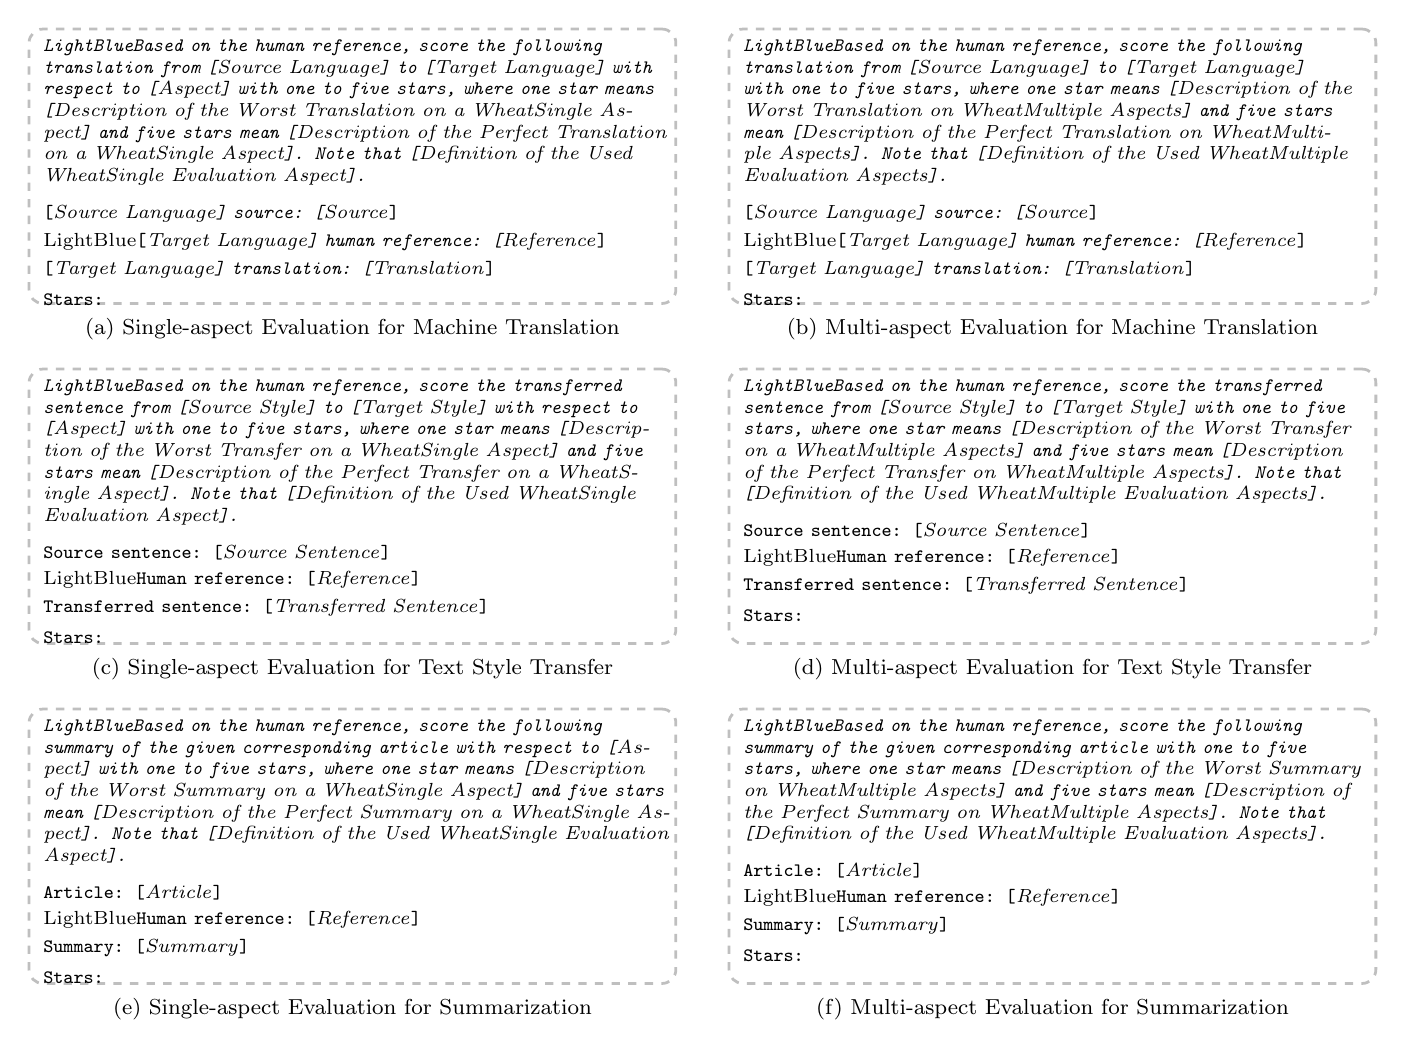
\begin{tikzpicture}
        \scriptsize{
			\begin{scope}[]
				
				\node [anchor=north,rectangle,rounded corners=5pt,minimum height=1.4in, minimum width=3.3in, line width=1pt, draw=lightgray, dashed] (box) at (0, 0) {};
				
				\node [anchor=north, text width=3.2in] (p1) at ([xshift=0.2em, yshift=-0.2em]box.north) {\textit{\texttt{\sethlcolor{LightBlue}\hl{Based on the human reference}, score the following translation from [}Source Language\texttt{] to [}Target Language\texttt{] with respect to [}Aspect\texttt{] with one to five stars, where one star means [}Description of the Worst Translation on a \sethlcolor{Wheat}\hl{Single Aspect}\texttt{] and five stars mean [}Description of the Perfect Translation on a \sethlcolor{Wheat}\hl{Single Aspect}\texttt{]. Note that [}Definition of the Used \sethlcolor{Wheat}\hl{Single Evaluation Aspect}\texttt{].}}};
				
				\node [anchor=north, text width=3.2in] (p2) at ([xshift=0em, yshift=-0.2em]p1.south) {\texttt{[}\textit{Source Language\texttt{] source: [}Source}\texttt{]}};
				
				\node [anchor=north, text width=3.2in] (p3) at ([xshift=0em, yshift=0.2em]p2.south) {\sethlcolor{LightBlue}\hl{\texttt{[}\textit{Target Language\texttt{] human reference: [}Reference}\texttt{]}}};
				
				\node [anchor=north, text width=3.2in] (p4) at ([xshift=0em, yshift=0.2em]p3.south) {\texttt{[}\textit{Target Language\texttt{] translation: [}Translation}\texttt{]}};
				
				\node [anchor=north, text width=3.2in] (p5) at ([xshift=0em, yshift=0em]p4.south) {\texttt{Stars:}};
				
				\footnotesize{
					\node [anchor=north] (title) at ([xshift=0em, yshift=-0.2em]box.south) {(a) Single-aspect Evaluation for Machine Translation};
				}
			\end{scope}
		}
		
		\scriptsize{
			\begin{scope}[xshift=3.5in]
				
				\node [anchor=north,rectangle,rounded corners=5pt,minimum height=1.4in, minimum width=3.3in, line width=1pt, draw=lightgray, dashed] (box) at (0, 0) {};
				
				\node [anchor=north, text width=3.2in] (p1) at ([xshift=0.2em, yshift=-0.2em]box.north) {\textit{\texttt{\sethlcolor{LightBlue}\hl{Based on the human reference}, score the following translation from [}Source Language\texttt{] to [}Target Language\texttt{] with one to five stars, where one star means [}Description of the Worst Translation on  \sethlcolor{Wheat}\hl{Multiple Aspects}\texttt{] and five stars mean [}Description of the Perfect Translation on \sethlcolor{Wheat}\hl{Multiple Aspects}\texttt{]. Note that [}Definition of the Used \sethlcolor{Wheat}\hl{Multiple Evaluation Aspects}\texttt{].}}};
				
				\node [anchor=north, text width=3.2in] (p2) at ([xshift=0em, yshift=-0.2em]p1.south) {\texttt{[}\textit{Source Language\texttt{] source: [}Source}\texttt{]}};
				
				\node [anchor=north, text width=3.2in] (p3) at ([xshift=0em, yshift=0.2em]p2.south) {\sethlcolor{LightBlue}\hl{\texttt{[}\textit{Target Language\texttt{] human reference: [}Reference}\texttt{]}}};
				
				\node [anchor=north, text width=3.2in] (p4) at ([xshift=0em, yshift=0.2em]p3.south) {\texttt{[}\textit{Target Language\texttt{] translation: [}Translation}\texttt{]}};
				
				\node [anchor=north, text width=3.2in] (p5) at ([xshift=0em, yshift=0em]p4.south) {\texttt{Stars:}};
				
				\footnotesize{
					\node [anchor=north] (title) at ([xshift=0em, yshift=-0.2em]box.south) {(b) Multi-aspect Evaluation for Machine Translation};
				}
			\end{scope}
		}
    \scriptsize{
			\begin{scope}[yshift=-1.7in]
				
				\node [anchor=north,rectangle,rounded corners=5pt,minimum height=1.4in, minimum width=3.3in, line width=1pt, draw=lightgray, dashed] (box) at (0, 0) {};
				
				\node [anchor=north, text width=3.2in] (p1) at ([xshift=0.2em, yshift=-0.2em]box.north) {\textit{\texttt{\sethlcolor{LightBlue}\hl{Based on the human reference}, score the transferred sentence from [}Source Style\texttt{] to [}Target Style\texttt{] with respect to [}Aspect\texttt{] with one to five stars, where one star means [}Description of the Worst Transfer on a \sethlcolor{Wheat}\hl{Single Aspect}\texttt{] and five stars mean [}Description of the Perfect Transfer on a \sethlcolor{Wheat}\hl{Single Aspect}\texttt{]. Note that [}Definition of the Used \sethlcolor{Wheat}\hl{Single Evaluation Aspect}\texttt{].}}};
				
				\node [anchor=north, text width=3.2in] (p2) at ([xshift=0em, yshift=-0.2em]p1.south) {\texttt{Source sentence: [}\textit{Source Sentence}\texttt{]}};
				
				\node [anchor=north, text width=3.2in] (p3) at ([xshift=0em, yshift=0.2em]p2.south) {\sethlcolor{LightBlue}\hl{\texttt{Human reference: [}\textit{Reference}\texttt{]}}};
				
				\node [anchor=north, text width=3.2in] (p4) at ([xshift=0em, yshift=0.2em]p3.south) {\texttt{Transferred sentence: [}\textit{Transferred Sentence}\texttt{]}};
				
				\node [anchor=north, text width=3.2in] (p5) at ([xshift=0em, yshift=0em]p4.south) {\texttt{Stars:}};
				
				\footnotesize{
					\node [anchor=north] (title) at ([xshift=0em, yshift=-0.2em]box.south) {(c) Single-aspect Evaluation for Text Style Transfer};
				}
			\end{scope}
		}

    \scriptsize{
			\begin{scope}[xshift=3.5in, yshift=-1.7in]
				
				\node [anchor=north,rectangle,rounded corners=5pt,minimum height=1.4in, minimum width=3.3in, line width=1pt, draw=lightgray, dashed] (box) at (0, 0) {};
				
				\node [anchor=north, text width=3.2in] (p1) at ([xshift=0.2em, yshift=-0.2em]box.north) {\textit{\texttt{\sethlcolor{LightBlue}\hl{Based on the human reference}, score the transferred sentence from [}Source Style\texttt{] to [}Target Style\texttt{] with one to five stars, where one star means [}Description of the Worst Transfer on a \sethlcolor{Wheat}\hl{Multiple Aspects}\texttt{] and five stars mean [}Description of the Perfect Transfer on \sethlcolor{Wheat}\hl{Multiple Aspects}\texttt{]. Note that [}Definition of the Used \sethlcolor{Wheat}\hl{Multiple Evaluation Aspects}\texttt{].}}};
				
				\node [anchor=north, text width=3.2in] (p2) at ([xshift=0em, yshift=-0.2em]p1.south) {\texttt{Source sentence: [}\textit{Source Sentence}\texttt{]}};
				
				\node [anchor=north, text width=3.2in] (p3) at ([xshift=0em, yshift=0.2em]p2.south) {\sethlcolor{LightBlue}\hl{\texttt{Human reference: [}\textit{Reference}\texttt{]}}};
				
				\node [anchor=north, text width=3.2in] (p4) at ([xshift=0em, yshift=0.2em]p3.south) {\texttt{Transferred sentence: [}\textit{Transferred Sentence}\texttt{]}};
				
				\node [anchor=north, text width=3.2in] (p5) at ([xshift=0em, yshift=0em]p4.south) {\texttt{Stars:}};
				
				\footnotesize{
					\node [anchor=north] (title) at ([xshift=0em, yshift=-0.2em]box.south) {(d) Multi-aspect Evaluation for Text Style Transfer};
				}
			\end{scope}
		}
  	\scriptsize{
			\begin{scope}[yshift=-3.4in]
				
				\node [anchor=north,rectangle,rounded corners=5pt,minimum height=1.4in, minimum width=3.3in, line width=1pt, draw=lightgray, dashed] (box) at (0, 0) {};
				
				\node [anchor=north, text width=3.2in] (p1) at ([xshift=0.2em, yshift=-0.2em]box.north) {\textit{\texttt{\sethlcolor{LightBlue}\hl{Based on the human reference}, score the following summary of the given corresponding article with respect to [}Aspect\texttt{] with one to five stars, where one star means [}Description of the Worst Summary on a \sethlcolor{Wheat}\hl{Single Aspect}\texttt{] and five stars mean [}Description of the Perfect Summary on a \sethlcolor{Wheat}\hl{Single Aspect}\texttt{]. Note that [}Definition of the Used \sethlcolor{Wheat}\hl{Single Evaluation Aspect}\texttt{].}}};
				
				\node [anchor=north, text width=3.2in] (p2) at ([xshift=0em, yshift=-0.2em]p1.south) {\texttt{Article: [}\textit{Article}\texttt{]}};
				
				\node [anchor=north, text width=3.2in] (p3) at ([xshift=0em, yshift=0.2em]p2.south) {\sethlcolor{LightBlue}\hl{\texttt{Human reference: [}\textit{Reference}\texttt{]}}};
				
				\node [anchor=north, text width=3.2in] (p4) at ([xshift=0em, yshift=0.2em]p3.south) {\texttt{Summary: [}\textit{Summary}\texttt{]}};
				
				\node [anchor=north, text width=3.2in] (p5) at ([xshift=0em, yshift=0em]p4.south) {\texttt{Stars:}};
				
				\footnotesize{
					\node [anchor=north] (title) at ([xshift=0em, yshift=-0.2em]box.south) {(e) Single-aspect Evaluation for Summarization};
				}
			\end{scope}
		}
		
		\scriptsize{
			\begin{scope}[xshift=3.5in,yshift=-3.4in]
				
				\node [anchor=north,rectangle,rounded corners=5pt,minimum height=1.4in, minimum width=3.3in, line width=1pt, draw=lightgray, dashed] (box) at (0, 0) {};
				
				\node [anchor=north, text width=3.2in] (p1) at ([xshift=0.2em, yshift=-0.2em]box.north) {\textit{\texttt{\sethlcolor{LightBlue}\hl{Based on the human reference}, score the following summary of the given corresponding article with one to five stars, where one star means [}Description of the Worst Summary on \sethlcolor{Wheat}\hl{Multiple Aspects}\texttt{] and five stars mean [}Description of the Perfect Summary on \sethlcolor{Wheat}\hl{Multiple Aspects}\texttt{]. Note that [}Definition of the Used \sethlcolor{Wheat}\hl{Multiple Evaluation Aspects}\texttt{].}}};
				
				\node [anchor=north, text width=3.2in] (p2) at ([xshift=0em, yshift=-0.2em]p1.south) {\texttt{Article: [}\textit{Article}\texttt{]}};
				
				\node [anchor=north, text width=3.2in] (p3) at ([xshift=0em, yshift=0.2em]p2.south) {\sethlcolor{LightBlue}\hl{\texttt{Human reference: [}\textit{Reference}\texttt{]}}};
				
				\node [anchor=north, text width=3.2in] (p4) at ([xshift=0em, yshift=0.2em]p3.south) {\texttt{Summary: [}\textit{Summary}\texttt{]}};
				
				\node [anchor=north, text width=3.2in] (p5) at ([xshift=0em, yshift=0em]p4.south) {\texttt{Stars:}};
				
				\footnotesize{
					\node [anchor=north] (title) at ([xshift=0em, yshift=-0.2em]box.south) {(f) Multi-aspect Evaluation for Summarization};
				}
			\end{scope}
		}
	\end{tikzpicture}
        \vspace{-2mm}
	\caption{
	    Prompt templates of the single and multi-aspect evaluation.
		Single-aspect evaluation means that the model only needs to consider a specific aspect during the evaluation process.
		Conversely, multi-aspect evaluation means that the model must consider multiple aspects concurrently, e.g., simultaneously considering meaning preservation and grammar to assign stars. Template portions \sethlcolor{LightBlue}\hl{highlighted in blue} denote the reference input used only by reference-based evaluation, and that those \sethlcolor{Wheat}\hl{highlighted in yellow} denote the differentiation between single-aspect evaluation and multi-aspect evaluation.
	}
        \vspace{-4mm}
	\label{fig:prompt}
\end{figure*}